\documentclass[11pt]{article}
\usepackage[T1]{fontenc}
\usepackage[utf8]{inputenc}
\usepackage{lmodern}
\usepackage[margin=1in]{geometry}
\usepackage{amsmath,amssymb,amsthm,mathtools}
\usepackage{booktabs,array}
\usepackage{microtype}
\usepackage{xcolor}
\usepackage{tikz}
\usetikzlibrary{arrows.meta,calc,patterns}
\usepackage[colorlinks=true,linkcolor=blue!45!black,citecolor=blue!45!black,urlcolor=blue!45!black]{hyperref}
\hypersetup{pdftitle={A Torsion-Free Group Algebra with Zero Divisors},pdfauthor={OpenAI}}
\usepackage[capitalise,noabbrev]{cleveref}
\usepackage{enumitem}
\setlist[itemize]{topsep=4pt,itemsep=2pt}
\setlist[enumerate]{topsep=4pt,itemsep=2pt}
\setlength{\emergencystretch}{2em}
\newtheorem{theorem}{Theorem}[section]
\newtheorem{proposition}[theorem]{Proposition}
\newtheorem{lemma}[theorem]{Lemma}
\newtheorem{corollary}[theorem]{Corollary}
\newtheorem{claim}[theorem]{Claim}
\theoremstyle{definition}
\newtheorem{definition}[theorem]{Definition}
\newtheorem{remark}[theorem]{Remark}
\AddToHook{env/theorem/begin}{\crefalias{theorem}{theorem}}
\AddToHook{env/proposition/begin}{\crefalias{theorem}{proposition}}
\AddToHook{env/lemma/begin}{\crefalias{theorem}{lemma}}
\AddToHook{env/corollary/begin}{\crefalias{theorem}{corollary}}
\AddToHook{env/claim/begin}{\crefalias{theorem}{claim}}
\AddToHook{env/definition/begin}{\crefalias{theorem}{definition}}
\AddToHook{env/remark/begin}{\crefalias{theorem}{remark}}
\numberwithin{equation}{section}
\DeclareMathOperator{\girth}{girth}
\DeclareMathOperator{\diam}{diam}
\DeclareMathOperator{\dist}{dist}
\DeclareMathOperator{\supp}{supp}
\title{A Torsion-Free Group Algebra with Zero Divisors}
\author{OpenAI}
\date{September 23, 2026}
\begin{document}
\maketitle
\begin{abstract}
We disprove Kaplansky's zero-divisor conjecture by constructing a finitely presented torsion-free group \(G\) for which \(\mathbb F_2[G]\) has nonzero zero divisors. The group admits a finite two-dimensional classifying space.
\end{abstract}

\section{Introduction}\label{sec:introduction}

Kaplansky's zero-divisor conjecture asserts that \(K[G]\) has no nonzero zero divisors whenever \(K\) is a field and \(G\) is torsion-free. Here \(K[G]\) is the algebra of finite formal sums of elements of \(G\), with multiplication extended bilinearly from the group law. We prove the following negative resolution.

\begin{theorem}\label{thm:main}
There exist a finitely presented torsion-free group \(G\) and nonzero elements
\(\alpha,\beta\in\mathbb F_2[G]\) such that \(\alpha\beta=0\).
Moreover, \(G\) admits a finite two-dimensional classifying space.
\end{theorem}

\subsection*{History and related constructions}

The question goes back to Higman's 1940 thesis~\cite{Higman1940Thesis}; its conjectural formulation is reproduced by Sandling~\cite[p.~112]{Sandling1981}. It was also posed in Kaplansky's 1956 conference contribution, published in 1957~\cite[Problem~6]{Kaplansky1957}; see the historical discussion in~\cite{Gardam2021}. Finite-order elements give elementary zero divisors: if \(g\) has order \(m>1\), then \((1-g)(1+g+\cdots+g^{m-1})=0\). The conjecture asks whether removing this obstruction suffices.

Substantial positive results explain why torsion-freeness is a natural dividing line. Higman proved the domain conclusion for groups in which every nontrivial subgroup maps onto \(\mathbb Z\)~\cite[Section~4, Theorems~12--13]{Higman1940}. Kropholler, Linnell, and Moody established it for torsion-free elementary amenable groups, even with division-ring coefficients~\cite[Theorem~1.4]{KrophollerLinnellMoody1988}. More recently, Fisher and S\'anchez-Peralta obtained division-ring embeddings for group algebras of torsion-free virtually compact special groups and torsion-free compact \(3\)-manifold groups, and the domain conclusion for torsion-free \(3\)-manifold groups without a finite-generation assumption~\cite[Theorem~1.3 and Corollary~1.5]{FisherSanchezPeralta2026}. These results concern particular classes of groups; our construction uses a different geometric mechanism.

A group has the \emph{unique-product property} if, for every pair of finite nonempty subsets \(P,Q\), some element of \(PQ\) has exactly one expression \(pq\) with \(p\in P\), \(q\in Q\). Applying this property to the supports of two nonzero group-algebra elements gives a nonzero product coefficient. Rips and Segev constructed torsion-free groups without unique product~\cite{RipsSegev1987}; Steenbock supplied a graphical small-cancellation treatment of their construction~\cite{Steenbock2015}. Mian and Siddique report a machine-checked non-unique-product witness for Gardam's \(\widetilde A_2\) lattice, taking torsion-freeness from Gardam rather than formalizing it~\cite[Sections~1 and~7]{MianSiddique2026}. Failure of unique product alone does not produce a zero divisor: over \(\mathbb F_2\), the relevant representation counts must be even, not merely greater than one.

The distinct \emph{unit conjecture} asks whether, for a torsion-free group \(G\) and a field \(K\), every unit of \(K[G]\) is a nonzero scalar multiple of a group element. Gardam disproved it over \(\mathbb F_2\)~\cite{Gardam2021} and subsequently over \(\mathbb C\)~\cite{Gardam2024}; a nontrivial unit is not a zero divisor.

Mineyev developed product structures and sufficient geometric criteria for obtaining nontrivial zero divisors or units in torsion-free group algebras over \(\mathbb F_2\)~\cite[Theorem~27]{Mineyev2024}. Garg and Mineyev study these criteria through finite-support combinatorics and computation~\cite[Theorems~1--3 and~16]{GargMineyev2025}. Shin proves that the orientable no-fold, triple-girth route cannot succeed when both support sizes are at least two~\cite[Theorem~1.1 and Corollary~1.2]{Shin2026}; this obstruction does not address the arrangement-exclusion argument here. Our construction supplies its own coefficient cancellation, root separation, and torsion-freeness proofs rather than applying those geometric criteria.

\subsection*{The cancellation mechanism and the two safeguards}

We use two finite graphs \(\Gamma_A,\Gamma_B\) immersed into one rose \(F\), a graph with one vertex and one edge for each generator. Every edge is read with a signed label, reversed when its orientation is reversed. Choose roots \(x_A,x_B\), and let \(A',B'\) be the full vertex sets of their connected components. Attach an abstract cone on each graph component along its labelled map to \(F\), obtaining a complex \(X\), and put \(G=\pi_1(X)\). Coning kills the labels of all closed graph paths. Thus a path from \(x_A\) to \(x\in A'\) has a well-defined label \(g_x\in G\), independent of the chosen path; define \(h_y\) from \(x_B\) to \(y\in B'\) in the same way. The proposed factors are
\begin{equation}\label{eq:overview-factors}
 \alpha=\sum_{x\in A'}g_x,\qquad
 \beta=\sum_{y\in B'}h_y^{-1}\quad\text{in }\mathbb F_2[G].
\end{equation}

Let \(S_x\) and \(S_y\) be the outgoing signed-label sets. We prescribe them so that \(|S_x\cap S_y|\) is odd for every pair. Form a graph on \(A'\times B'\) by simultaneous steps of a common label \(t\). Along each step the product is unchanged, since
\begin{equation}\label{eq:overview-common-step}
 (g_xt)(h_yt)^{-1}=g_xh_y^{-1}.
\end{equation}
Every vertex of this finite graph has odd degree \(|S_x\cap S_y|\). Hence each connected component has even cardinality, by the degree-sum formula. Its vertices all contribute the same group element to \(\alpha\beta\), so their contributions cancel in characteristic two.

This simple cancellation leaves two substantial safeguards. First, both factors must survive in the quotient: we prove that a path from either prescribed root to any different vertex in its component has nontrivial label. The root is then the only contributor to the identity coefficient in each factor, so both are nonzero. We do not need to distinguish labels of two non-root vertices. Second, the quotient group must be torsion-free: we prove that \(X\) is aspherical, making it a finite two-dimensional classifying space and ruling out torsion. Both safeguards will follow by excluding certain planar configurations of paired path occurrences.

\subsection*{From random graphs to topological control}

The outgoing-label types use lines in a finite projective plane together with three extra letters. Their cross-intersections force parity, while their turn frequencies satisfy an exponentially decaying squared-word estimate. We convert this estimate into an exclusion of bounded systems of almost completely paired paths. Paths may traverse the same edge repeatedly; multiplicity stages keep track of those repeated uses, while nearly aligned blocks control comparisons of arbitrary subpaths. Multiplying numerical expectation bounds selects one stage with a small expected count, without asserting independence between stages.

The remaining obstacle is that a sphere can involve arbitrarily many paths of arbitrarily large total length. Lipton--Tarjan planar separation~\cite{LiptonTarjan1979} reduces each such configuration to a bounded system. Long boundaries are first split and closed at a controlled cost, and planar gap counting bounds the number of comparison intervals after localization. The proportion of unpaired positions allowed by the probabilistic estimate is fixed before the bounds on the number and lengths of paths. This order permits the same bounded class to detect every large spherical arrangement, rather than a union bound over all arrangement sizes.

Graphical small cancellation provides important antecedents for this strategy. Gromov's random graphical presentations connect word-coincidence estimates with geometric control~\cite{Gromov2003}; Ollivier and Gruber develop precise graphical criteria for graph embeddings and asphericity~\cite{Ollivier2006,Gruber2015}. Distinguishing genuinely different graph lifts from coincident lifts is central to these arguments and to Bereznyuk's spherical-diagram approach~\cite{Bereznyuk2019}. Here the prescribed vertex types and repeated traversals require a separate probability estimate, and the needed topology is proved directly by cone-picture surgery. We do not invoke a small-cancellation or \(\mathrm{CAT}(0)\) criterion for these graphs.

\subsection*{Conventions and proof structure}

All graphs are finite unless stated otherwise. A graph may initially have loops or parallel edges; both are counted in its girth. A signed alphabet \(T\) has a fixed-point-free involution \(t\mapsto\bar t\), with \(\bar t\) denoting the inverse letter. The rose \(F\) has one vertex and one unoriented edge for each inverse pair. A labelled graph maps immersively to \(F\) when each outgoing label occurs at most once at each vertex. An \emph{immersed path} is an edge path with no immediate reversal; a closed path is \emph{cyclically immersed} if this also holds at its last/first junction. Length always counts edge traversals, including repetitions.

\Cref{sec:types,sec:bounded-pattern} construct the random graphs and rule out bounded patterns. \Cref{sec:planar} extracts such a pattern from every reduced spherical arrangement. \Cref{sec:topology} explains why either an essential sphere or a trivial label on a path from a prescribed root to a different vertex would produce such an arrangement. \Cref{sec:factors} uses the resulting asphericity and root separation to complete the factor construction and prove \Cref{thm:main}. All logarithms are natural. Constants in asymptotic estimates are independent of the sampling size \(n\); additional fixed parameters on which they depend will be indicated.

\section{Prescribed types and random matchings}\label{sec:types}

We construct the two immersed graphs so that their outgoing-label sets
have odd cross-intersections, the condition needed for cancellation.
The same vertex types also provide a squared-word decay estimate.
Conditioning the matchings on large girth will preserve enough control
to prove a diameter bound and, in \Cref{sec:bounded-pattern}, exclude
the path configurations that could defeat the geometric safeguards.

\subsection{The finite geometry}

Fix
\[
q=128,\qquad v=q^2+q+1=16513,\qquad p=\frac{q+1}{v}.
\]
The projective plane over \(\mathbb F_q\) has \(v\) points and \(v\) lines. Each line has \(q+1\) points, each point lies on \(q+1\) lines, two distinct points lie on one common line, and two distinct lines meet at one point. These facts follow by counting one- and two-dimensional subspaces of \(\mathbb F_q^3\).

Let \(T\) consist of its \(v\) points, called \emph{ordinary letters}, and three further \emph{extra letters}. Pair the extras with three distinct ordinary letters, and pair the remaining ordinary letters arbitrarily in twos. This defines a fixed-point-free involution on \(T\), since \(v-3\) is even. In particular, \(|T|=16516\), and the corresponding rose has \(8258\) edges.

Take disjoint vertex sets \(A,B\), each of size \(n\). For each vertex \(x\), prescribe a set \(S_x\subset T\) of outgoing labels as follows:
\begin{enumerate}
\item On either side the ordinary part of \(S_x\) is a line, with every line represented equally often.
\item Within each line class on \(A\), the extra part is each of the three two-element subsets with proportion \(p/2\) apiece, and is otherwise empty.
\item Within each line class on \(B\), the extra part is all three extras with proportion \(p\), and is otherwise empty.
\end{enumerate}
These are exact empirical proportions. We take \(n\to\infty\) through multiples of \(2v^2\), so all counts are integral. For example, at \(n=2v^2\), each line class on \(A\) has \(129\) vertices of each double-extra type and \(32639\) of the empty type; on \(B\) it has \(258\) of the triple-extra type and \(32768\) of the empty type.

Every letter has frequency \(p\) on each side. Two ordinary line parts meet in either \(1\) or \(q+1=129\) points. An extra part on \(A\) meets an extra part on \(B\) in either \(0\) or \(2\) letters. Thus
\begin{equation}\label{eq:odd-intersections}
 |S_x\cap S_y|\ \text{is odd for every }x\in A,\ y\in B.
\end{equation}
Thus the parity condition is built into the types, independently of
how their edges will be matched. The random choice can now be used
entirely to control the geometry without risking this condition.

Choose two vertices \(x_A\in A\) and \(x_B\in B\) in advance. For \(Y=A,B\), write
\[
Y_t=\{x\in Y:t\in S_x\},\qquad |Y_t|=np.
\]
For each inverse pair, choose a bijection \(Y_t\to Y_{\bar t}\), using its inverse for the opposite direction. A matched pair gives an edge labelled \(t\) in one direction and \(\bar t\) in the other. Do this independently for all inverse pairs and both sides before any conditioning. The resulting graphs are denoted
\[
\Gamma_A,\quad\Gamma_B,\qquad
\Gamma=\Gamma_A\sqcup\Gamma_B.
\]
They immerse into \(F\), since every outgoing letter occurs once at each vertex that carries it. Their degrees lie between \(q+1\) and
\(d_*=q+4=132\).
A prescription for one matching edge can be described using either orientation. Whenever prescriptions are counted, an edge and its reverse describe a single prescription.

\subsection{Turn weights}

For a non-cancelling turn \(t,u\), let \(w(t,u)\) be the frequency of \(u\) among the vertices of \(B\) that contain \(\bar t\). Put \(w(t,\bar t)=0\). The corresponding conditional frequency on \(A\) is at most \(w(t,u)\). Indeed, for distinct \(\bar t,u\), the weights on \(B\) are
\[
\begin{array}{c|ccc}
(\bar t,u)&\text{ordinary, ordinary}&
\text{ordinary, extra}&\text{extra, extra}\\ \hline
w(t,u)&1/(q+1)&p&1.
\end{array}
\]
The mixed entry is symmetric; the extra-extra frequency on \(A\) is \(1/2\). In particular, every positive weight lies in \([1/129,1]\).

For a word \(W=t_1\cdots t_h\), define
\begin{equation}\label{eq:word-weight}
P(W)=\prod_{i=1}^{h-1}w(t_i,t_{i+1}).
\end{equation}
Write \(W^{-1}=\bar t_h\cdots\bar t_1\). Equal letter marginals and symmetry of joint incidence give
\begin{equation}\label{eq:reversal-weight}
w(t,u)=w(\bar u,\bar t),\qquad P(W)=P(W^{-1}).
\end{equation}
For non-cancelling turns this follows by dividing the joint frequency of
\(\bar t,u\) by \(p\); for cancelling turns both weights in the first equality are zero.

\begin{lemma}\label{lem:squared-words}
There is a constant \(\delta>0\) such that, for every sufficiently large \(h\),
\begin{equation}\label{eq:squared-words}
 \sum_{W\in T^h}P(W)^2\le e^{-2\delta h}.
\end{equation}
\end{lemma}
\begin{proof}
Let \(M_{t,u}=w(t,u)^2\), and set \(f(t)=5\) if \(\bar t\) is extra and \(f(t)=1\) otherwise. There are precisely three states of weight five.

If \(\bar t\) is ordinary, the ordinary successors different from \(\bar t\) contribute \((v-1)/(q+1)^2=q/(q+1)\) before the weights \(f\) are inserted. At most three such successors have their weight increased by four. The extra successors all have weight one. Hence
\[
(Mf)(t)\le\frac{q}{q+1}+3p^2+\frac{12}{(q+1)^2}
 =\frac{500731261911}{504183783481}<\frac{149}{150}.
\]
If \(\bar t\) is extra, the other two extras contribute two; the ordinary successors contribute at most \(vp^2+12p^2\). Thus
\[
\frac{(Mf)(t)}{f(t)}
 \le\frac{2+vp^2+12p^2}{5}
 =\frac{820350863}{1363395845}<\frac{149}{150}.
\]
Consequently \(Mf\le(149/150)f\). Since \(\mathbf1\le f\) and
\(\sum_t f(t)=16528<e^{10}\),
\[
\sum_{W\in T^h}P(W)^2
=\mathbf1^{\mathsf T}M^{h-1}\mathbf1
\le16528(149/150)^{h-1}
\le e^{-h/300}\qquad(h\ge3002).
\]
For example, \(\delta=1/600\) is admissible.
\end{proof}

\subsection{Girth conditioning and switching}

Fix a sufficiently small positive constant \(c\), and put
\[
L=\lfloor c\log n\rfloor.
\]
It is enough that
\begin{equation}\label{eq:c-choice}
 c\log(2|T|/p)<1,\qquad 2c\log d_*<1;
\end{equation}
one may take \(c=1/100\). We work with the uniform tuple of matchings conditioned on \(\girth(\Gamma)\ge L\). The next lemma both justifies this conditioning and gives a bound within the conditioned space.

\begin{lemma}\label{lem:prescriptions}
For all sufficiently large admissible \(n\), there is a tuple of matchings with \(\girth(\Gamma)\ge L\).
In the uniform distribution on such tuples, condition further on any feasible set of \(s\) prescribed matching pairs. The probability of an additional specified pair, not already prescribed in either direction, is at most
\begin{equation}\label{eq:prescription-bound}
 \frac{1}{np-s-r_n},
 \qquad r_n=O(d_*^{2L+2})=o(n),
\end{equation}
whenever the denominator is positive.
The error \(r_n\) can be chosen uniformly over all prescriptions.
\end{lemma}
\begin{proof}
Before girth conditioning, a feasible simple cycle of length \(k<L\) has at most \(2n^k|T|^k\) vertex-and-letter descriptions. Its distinct edges require \(k\) distinct matching prescriptions, with probability at most \((np-k)^{-k}\). Thus the expected number of edges lying on cycles shorter than \(L\) is at most
\[
2\sum_{k<L}k\,n^k|T|^k(np-k)^{-k}
 \le2\sum_{k<L}k(2|T|/p)^k=o(n)
\]
for sufficiently large \(n\), by \eqref{eq:c-choice}. Choose a tuple with \(o(n)\) such \emph{bad edges}.

Let \(xy\) be a bad edge, oriented with label \(t\). Among the \(np\) edges for this inverse pair on the same side, choose an edge \(uz\), also oriented with label \(t\), that is not bad and whose endpoint set is at distance greater than \(2L\) from \(\{x,y\}\). This is possible: bad edges exclude \(o(n)\) choices, and the maximum-degree ball bound excludes another \(O(d_*^{2L+2})=o(n)\).

Transpose the two matches, replacing \(xy,uz\) by \(xz,uy\). A short cycle using only one new edge would give an old path between the distant endpoint sets. If a short cycle uses both, deleting them leaves old paths pairing the endpoints as either \((x,u),(y,z)\) or \((x,y),(u,z)\). The first case again joins the distant sets. In the second, the \(u\)-to-\(z\) path together with \(uz\) is an old short cycle, contradicting the choice of \(uz\). This includes \(x=y\), when the \(x\)-to-\(y\) path may have length zero. No short cycle is created. The chosen bad edge disappears, and the other removed edge was not bad, so the number of bad edges strictly decreases. Repetition produces a tuple of girth at least \(L\).

Now restrict to any feasible girth-conditioned set with \(s\) previous prescriptions, and consider an additional compatible pair \(xy\). If it is incompatible, its probability is zero. From every tuple containing \(xy\), perform the same transposition with any sufficiently distant edge \(uz\) of the same inverse pair and side that is not previously prescribed. All edges are now nonbad. At least \(np-s-r_n\) choices are available, with one uniform ball-size error \(r_n\). Each output preserves girth and all prior prescriptions.

Given an output and the pair \(xy\) to restore, the inverse operation is unique: the current match of \(x\) is \(z\), and the current preimage of \(y\) is \(u\). Thus the map from a tuple containing \(xy\), together with an admissible transposition, to its output tuple is injective. If \(\Omega_s\) is the conditioned set and \(\Omega_{s,xy}\) is its subset containing \(xy\), then
\[
|\Omega_{s,xy}|(np-s-r_n)\le|\Omega_s|.
\]
This proves \eqref{eq:prescription-bound}.
\end{proof}

In particular, any feasible collection of \(E=O(L)\) distinct edge prescriptions has conditional probability at most
\begin{equation}\label{eq:few-edge-bound}
 (np)^{-E}\exp(o(L)).
\end{equation}
This follows by applying \Cref{lem:prescriptions} successively. Uniformity of its error is important; no independence after conditioning is asserted.

\begin{lemma}\label{lem:diameter}
With conditional probability tending to one, every connected component of \(\Gamma\) has diameter at most \(D_0L\), for a fixed constant \(D_0\).
\end{lemma}
\begin{proof}
Fix a small positive \(\rho\). On either side, require every vertex set of size \(1\le k\le\rho n\) to grow to at least \(2k\) vertices on adjoining all its neighbors. A failure supplies a set of \(2k\) vertices containing at least
\[
r=\lceil(q+1)k/2\rceil
\]
distinct edges: all edges incident to the failing \(k\)-set lie in the larger set and are counted at most twice by its degree sum.

There are at most \((C_1n/k)^{2k}\) choices for the larger set. Its possible typed edge prescriptions number \(O(k^2)\); choosing an unordered \(r\)-subset costs at most \((C_1k)^r\). Decrease \(\rho\) so that \(r\le np/3\) throughout the range. For sufficiently large \(n\), \Cref{lem:prescriptions} then bounds the probability of all \(r\) prescriptions by \((2/(np))^r\). Hence the probability of a failure of size \(k\), on either side, is at most a fixed multiple of
\[
(C_1n/k)^{2k}(C_1k)^r(2/(np))^r
 \le \bigl(C_2(k/n)^{62.5}\bigr)^k,
\]
because \(64.5\le r/k\le65\). Choose \(\rho\) still smaller so that \(C_2\rho^{62.5}<1/2\). Summing over \(k\le\sqrt n\) gives \(o(1)\); the sum over larger \(k\le\rho n\) is at most \(n2^{-\sqrt n}\).

On the resulting expansion event, every ball reaches more than \(\rho n\) vertices in \(R=O(\log n)\) steps. Along a geodesic, centers separated by \(2R+1\) have disjoint radius-\(R\) balls. At most \(1/\rho\) such balls fit in one side. This bounds each component diameter by \(O(\log n)=O(L)\), with a fixed constant.
\end{proof}

\section{A bounded-pattern estimate}
\label{sec:bounded-pattern}

All probabilities in this section refer to the distribution conditioned on
\(\operatorname{girth}(\Gamma)\ge L\).  We retain the predetermined vertices
\(x_A\) and \(x_B\). The possible rooted interval will accommodate a
null-homotopy of a root-to-vertex path in \Cref{sec:topology}.

Consider finitely many positive-length paths in \(\Gamma\), all cyclically
immersed and closed except possibly one immersed interval path whose
initial vertex is \(x_A\) or \(x_B\).  An \emph{occurrence} means a position
on one of these paths; different occurrences may traverse the same edge.
A pairing by \emph{interval pairs} consists of disjoint occurrence
intervals, paired in twos by length-preserving interval isometries.  Even
when the two intervals lie on the same path, they are distinct and
disjoint as occurrence intervals.  An order-preserving comparison
requires equal signed letters, and an order-reversing comparison
requires inverse letters in opposite orders.  We impose the additional
reduction condition
\begin{equation}
 \text{paired occurrences traverse distinct underlying undirected
 edges of }\Gamma.
 \label{eq:edge-reduction}
\end{equation}
Positions outside the paired intervals are called \emph{unpaired}.

\begin{samepage}
\begin{proposition}[Bounded-pattern estimate]
\label{prop:bounded-pattern}
There is a constant \(\varepsilon>0\), depending only on the fixed types
and turn weights, with the following property.  For every fixed positive
integer \(K\), fixed real \(C\ge1\), and fixed nonnegative integer \(I\),
the conditional probability tends to zero that there exists a system as
above having at most \(K\) paths, total length \(H\) with
\[
 L\le H\le CL,
\]
at most \(I\) interval pairs, and \(b\) unpaired occurrences, where
\(b\le\varepsilon H\).  In particular, \(\varepsilon\) is chosen before
\(K,C,I\), and these three bounds are held fixed as \(n\) tends to
infinity through its admissible values.
\end{proposition}
\end{samepage}

We first describe the actual image of a candidate system by boundedly
many chains. Sorting its edges by traversal multiplicity gives stages
whose total vertex exponent is nonpositive. Nearly aligned blocks turn
the path pairings into word constraints controlled by the squared-word
estimate. Together, these bounds make the product of the stage expectation
bounds exponentially small. Every realization must occur at every stage,
so one small expectation bound suffices for the union bound.

\begin{proof}
Fix \(K,C,I\).  Constants implicit in this proof may depend on these
bounds, whereas the final choice of \(\varepsilon\) will not.  Every
\(o(L)\) or \(o(s)\) estimate below is uniform over the patterns with these
fixed bounds.  Cutting comparison intervals at the chosen indexing
starts of closed paths changes only a fixed bound on the number of
interval pairs, so we make these cuts at the outset.

By \eqref{eq:reversal-weight}, reversing a chain does not change its word
weight.

\subsection*{The image graph and multiplicity stages}
Let \(\Delta\) be the actual image subgraph of a proposed system.  It has
at most \(CL\) edges and girth at least \(L\).  Mark every path start and
end, and every vertex whose degree in \(\Delta\) differs from two.  We
first show that \(\Delta\) consists of a bounded number of chains between
marks, with disjoint unmarked degree-two interiors.  A chain is allowed
to return to its initial mark.

Repeatedly delete leaves and their incident edges, and discard any edgeless
remnants. This preserves cycle rank. Set aside the components of the resulting core that are
circles; there are at most \(C\), since each uses at least \(L\) edges.
Suppress all degree-two vertices in the remaining core.  The resulting
multigraph has minimum degree at least three; its edges have positive
integer lengths, whose sum is at most \(CL\).  Suppose it has \(r>0\)
edges.  Start a non-backtracking walk uniformly on its \(2r\) directed
edges, and at every subsequent step choose uniformly among the allowed
continuations.  Uniform measure on directed edges is stationary: a
given directed edge with origin \(z\) has \(\deg(z)-1\) allowed
predecessors, each contributing
\(1/[2r(\deg(z)-1)]\).  This calculation also applies to loops and
parallel edges, with degrees counted by half-edges.

The expected expanded length of a walk of \(k\) edges is therefore at
most \(kCL/r\).  At least half of the probability lies on walks of
expanded length at most \(2kCL/r\).  Each particular walk has
probability at most \((2r)^{-1}2^{-(k-1)}\), so there are at least
\(r2^{k-1}\) such short walks.  Choose \(k=O(\log(r+1))\) so that this
number exceeds \((2r)^2\).  There are at most \((2r)^2\) ordered pairs of
endpoint vertices.  Two distinct short walks consequently have the same
endpoints.  Their expansions are distinct reduced paths.  Their union
contains a cycle, since in a tree there is only one reduced path between
two specified vertices.  That cycle has length at most \(4kCL/r\).
Girth at least \(L\) implies \(r\le4Ck\), bounding \(r\) in terms of
\(C\) alone.  Thus the cycle rank of \(\Delta\) is bounded.

The graph \(\Delta\) has no isolated vertices and has at most two leaves.
Indeed, a cyclically immersed path cannot visit a leaf, and an immersed
interval path can visit one only at an endpoint.  If \(\beta\) is the
cycle rank and \(c_\Delta\) the number of components, the degree-sum
identity gives
\[
 \sum_{\deg(z)\ge3}(\deg(z)-2)
 =2\beta-2c_\Delta+\#\{z:\deg(z)=1\}.
\]
It follows that the number and total degrees of branching vertices are
bounded.  There are also only boundedly many path-start and path-end
marks.  Every component contains a path start.  Suppressing all remaining
unmarked degree-two vertices now proves the asserted bound on the
number of marked chains, including circle components.

Every path traverses whole marked chains.  Write \(m_e\) for the total
number of traversals of an undirected edge \(e\) by all the paths; it is
constant on each chain.  If one immersed path traverses the same
oriented edge twice, the gap between the two starting positions is at
least \(L\): the intervening segment is a nonempty reduced closed walk
and hence contains a cycle.  A path of length \(h\) thus traverses any
given oriented edge at most \(h/L+1\) times.  Summing over paths and the
two orientations yields
\begin{equation}
 m_e\le 2(H/L+K)\le2(C+K).
 \label{eq:entropy-multiplicity}
\end{equation}
Consequently the total number of chain traversals is bounded as well.

There are only polynomially many unlabelled patterns in \(L\).  To
specify one, give the bounded marked multigraph, the positive integer
length of each chain, the side \(A\) or \(B\) of each component, the
oriented chain sequence of each path, the designation and starting side
of the possible interval path, and the comparison endpoints and their
orientation data.  Each integer endpoint has \(O(L)\) choices and there
are boundedly many of them.  We retain only patterns satisfying
\eqref{eq:edge-reduction}.  Vertex names in \(A\) and \(B\), and signed
edge labels, are not included in this description.  Crucially, the
abstract graph so described is the actual image graph: its subsequent
realizations must be injective on vertices and edges.

\paragraph{Multiplicity stages and vertex exponents.}
The density-counting viewpoint of organizing constraints by multiplicity,
discussed by Ollivier \cite{Ollivier2005}, motivates the stage organization
and selection below.  The conditioned matching estimate for the dependent
graph paths in this model is developed locally.

For \(1\le j\le m_*:=\max_e m_e\), let \(\Delta_j\) consist of all edges
with \(m_e\ge j\), together with their incident vertices.  Denote its
edge and vertex counts by \(E_j\) and \(V_j\).  Let \(\iota\) be one if
the interval path is present and zero otherwise.  Then
\begin{equation}
 \sum_{j=1}^{m_*}E_j=H,\qquad
 \sum_{j=1}^{m_*}V_j
 =\sum_{z\in\Delta^{(0)}}\max_{e\ni z}m_e
 \le H+\iota.
 \label{eq:entropy-incidences}
\end{equation}
For the inequality, let \(a(z)\) count interval-path endpoints at \(z\),
with multiplicity.  At a vertex, all traversal incidences except these
endpoints are coupled into passages between distinct half-edges, by
immersion and cyclic immersion.  Thus the incidences on a half-edge
of maximum multiplicity must be coupled to incidences on other
half-edges, except for at most \(a(z)\) endpoints.  Hence
\[
 2\max_{e\ni z}m_e
 \le \sum_{\text{half-edges at }z}m_e+a(z).
\]
Summing this inequality proves \eqref{eq:entropy-incidences}, because the
half-edge sum is \(2H\) and \(\sum_z a(z)=2\iota\).

Set \(k_1=\iota\), and \(k_j=0\) for \(j>1\).  In stage one the initial
vertex of the interval path has its prescribed image, saving one factor
of \(n\).  We claim no such saving at later stages.  The exponent needed
below satisfies
\begin{equation}
 \sum_{j=1}^{m_*}(V_j-E_j-k_j)\le0.
 \label{eq:entropy-n-exponent}
\end{equation}
In the later realization count, the exponent \(V_j-E_j-k_j\) will
count vertex-image choices against edge-prescription costs.
Equation~\eqref{eq:entropy-n-exponent} therefore controls the total
power of \(n\) across the multiplicity stages.
The remaining task is to obtain exponential decay from the label
constraints; counting only distinct edges would lose the incidence
balance that makes these two estimates compatible.

\subsection*{Word constraints on aligned blocks}
The aim is a common subdivision for which each comparison carries almost
all positions of a block into a single partner block. Orient each marked chain of length \(\ell\), identify it with
\([0,\ell]\), and put its edge positions at half-integers.  Splitting
comparisons at chain-traversal boundaries gives boundedly many
subcomparisons of the form
\[
 x\longmapsto\sigma x+a,\qquad \sigma\in\{1,-1\},\quad a\in\mathbb Z.
\]
These maps compare particular occurrences of subchains.  Relative to
the chosen chain orientations, their label relations are equality when
\(\sigma=1\) and inverse equality when \(\sigma=-1\).

Pad the list of integer offsets by zeros to a fixed length \(d\ge1\).
Put
\[
 N=\left\lfloor L^{1/(2(d+1))}\right\rfloor,
 \qquad R=\lfloor\sqrt N\rfloor.
\]
The simultaneous pigeonhole principle gives an integer
\(1\le u\le N^d\) such that
\(\operatorname{dist}(ua/L,\mathbb Z)\le1/N\) for every offset \(a\).
For completeness, place the \(N^d+1\) vectors of fractional parts of
\(k(a_1/L,\ldots,a_d/L)\), for \(0\le k\le N^d\), in the \(N^d\)
cubes of side \(1/N\).  Subtracting two vectors in the same cube gives
the required \(u\).  Choose the least such \(u\), so all choices are
determined by the unlabelled pattern, and set \(s=L/(uR)\).  Uniformly in
that pattern,
\begin{equation}
 \frac{L}{N^{d+1/2}}\le s\le\frac{L}{R},\qquad
 \max_a\operatorname{dist}(a/s,\mathbb Z)\le\frac{R}{N}.
 \label{eq:entropy-grid}
\end{equation}
In particular, \(s\) tends to infinity at least as a fixed positive
power of \(L\), while \(s/L\) and all the distances in
\eqref{eq:entropy-grid} tend to zero.

On each chain use the full grid intervals \([ks,(k+1)s)\) contained in
\([0,\ell]\), for integers \(k\ge0\).  The half-integer edge positions
in such an interval form a \emph{full block}.  Index these blocks over
all of \(\Delta\) by \(i\).  Their lengths and multiplicities satisfy
\[
 h_i=s+O(1),\qquad m_i=m_e\quad\text{on their chains}.
\]
The remaining end fragment of a chain has \(O(s+1)\) positions.  Every
traversal of the same chain uses this same subdivision, also when read
backwards.

Here is the alignment consequence of \eqref{eq:entropy-grid}, including
reflections.  Write \(a=\nu s+r\), with \(\nu\in\mathbb Z\) and
\(|r|=o(s)\).  A translation sends the \(k\)-th real grid interval to
the \((k+\nu)\)-th interval shifted by \(r\).  A reflection sends it to
\[
 ((\nu-k-1)s+r,(\nu-k)s+r].
\]
Because \(a\) is integral, the isometry preserves the half-integer
lattice.  In either case its image overlaps the indicated partner
grid block in a contiguous string of at least \(s-|r|-2=s-o(s)\)
positions.  The reversed endpoint convention in the reflection costs
only a bounded number of positions.

Figure~\ref{fig:block-alignment} illustrates the translation case.
The grid belongs to the underlying chain, not to an individual path
traversal: repeated traversals use the same blocks but give distinct
block occurrences. This distinction will matter when occurrence
pairings are projected to links between underlying blocks.

\begin{figure}[htbp]
\centering
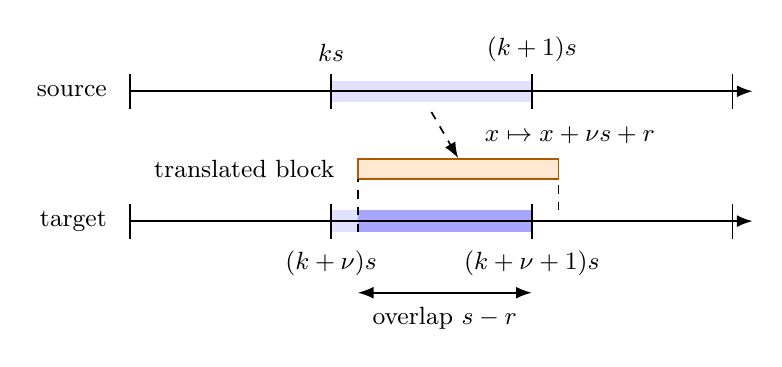
\begin{tikzpicture}[x=0.85cm,y=0.85cm,>=Latex,font=\small,line width=0.6pt]
\fill[blue!12] (3,1.8) rectangle (6,2.12);
\draw[->] (0,1.96)--(9.3,1.96);
\foreach \position in {0,3,6,9}
  \draw (\position,1.7)--(\position,2.22);
\node[anchor=south] at (3,2.25) {$ks$};
\node[anchor=south] at (6,2.25) {$(k+1)s$};
\node[anchor=east] at (-0.2,1.96) {source};
\draw[->,dashed] (4.5,1.65)--(4.9,0.96);
\node[anchor=west] at (5.15,1.3) {$x\mapsto x+\nu s+r$};
\fill[orange!18] (3.4,0.65) rectangle (6.4,0.95);
\draw[orange!70!black] (3.4,0.65) rectangle (6.4,0.95);
\node[anchor=east] at (3.2,0.8) {translated block};
\fill[blue!12] (3,-0.14) rectangle (6,0.18);
\fill[blue!35] (3.4,-0.14) rectangle (6,0.18);
\draw[->] (0,0.02)--(9.3,0.02);
\foreach \position in {0,3,6,9}
  \draw (\position,-0.24)--(\position,0.28);
\draw[dashed] (3.4,-0.14)--(3.4,0.65);
\draw[dashed] (6.4,0.18)--(6.4,0.65);
\node[anchor=east] at (-0.2,0.02) {target};
\node[anchor=north] at (3,-0.28) {$(k+\nu)s$};
\node[anchor=north] at (6,-0.28) {$(k+\nu+1)s$};
\draw[<->] (3.4,-1.05)--(6,-1.05);
\node[anchor=north] at (4.7,-1.12) {overlap $s-r$};
\end{tikzpicture}

\caption{Approximate alignment under a translation, shown schematically
with \(0<r=o(s)\). A source block is translated by \(a=\nu s+r\);
its image overlaps the indicated target block in real length \(s-r\).
Restricting to half-integer edge positions loses at most a bounded
number of positions, giving \(s-o(s)\) compared letters. The shift is
exaggerated for visibility. The proof also treats negative shifts and
reflections.}
\label{fig:block-alignment}
\end{figure}

Join two full-block occurrences whenever one of the subcomparisons
identifies contiguous subwords in them of length at least
\((1-\kappa)s\), where \(\kappa=o(1)\) is chosen uniformly large enough
to absorb the alignment and rounding errors.  Record one such substring
comparison with each join.  These joins form a partial matching of
block occurrences: each compared substring occupies more than half its
block, whereas the original comparison domains are disjoint as
occurrence intervals.  Thus a block occurrence cannot participate in
two joins.

Let \(b_*\) be the number of unmatched full-block occurrences.  Only
boundedly many blocks lie within \(3s+O(1)\) of a subcomparison cut or a
chain endpoint.  Away from these cuts, a full block in a comparison
domain has its partner full block and hence is matched.  Every remaining
unmatched block away from the cuts consists entirely of unpaired
positions.  There are \(O(L/s)\) block occurrences in total, so rounding
their lengths and charging the exceptional blocks gives
\begin{equation}
 sb_*\le b+O(s+L/s)=b+o(L).
 \label{eq:entropy-unmatched-blocks}
\end{equation}

\paragraph{Links between underlying blocks.}
Forget occurrence indices in this matching, obtaining a multigraph
whose vertices are the full blocks \(i\).  We call its edges
\emph{links} and include isolated blocks.  The substring positions and
directions attached to every link are already fixed by the unlabelled
pattern.  In a component \(\mathcal U\) of this link graph, a word on any
one block determines the word on each next block along a spanning tree
except for \(o(s)\) letters.  Indeed, the recorded comparison specifies
\(s-o(s)\) letters of the next word, possibly with reversal and
inversion.  Since the alphabet is fixed, the number of extensions of a
root word to all blocks in \(\mathcal U\) is at most
\begin{equation}
 \exp\bigl(o(s)|\mathcal U|\bigr).
 \label{eq:entropy-propagation}
\end{equation}
Additional links and immersion constraints can only reduce this number.

If \(\mathcal U\) has a self-link, choose a self-linked block as the
root. Its word has only \(\exp(o(s))\) possibilities, or the pattern is
infeasible. To prove this, first consider a translation self-link. Its
constraints have the form
\[
 W(x)=W(x+t)\quad(x\in D),
\]
where \(D\) and \(D+t\) are contiguous subsets of the same block and
\(|D|=s-o(s)\).  The integral shift \(t\) is nonzero by
\eqref{eq:edge-reduction}; a zero shift would compare the same underlying
edge with itself.  On the \(h_i\) positions of the block, the
\(|D|\) distinct constraint edges form a forest of arithmetic chains
with step \(|t|\).  Thus this forest has \(h_i-|D|=o(s)\) components,
leaving at most \(|T|^{h_i-|D|}=\exp(o(s))\) root words.

For a reflection self-link, write its map as \(\phi(x)=a-x\).  The
intersection \(J=D\cap\phi(D)\) of its nearly full domain and image is
a contiguous reflection-invariant set with
\(|J|\ge2|D|-h_i>0\).  If \(a\) is odd, its center is a half-integer
position in \(J\), forcing that letter to equal its inverse.  If \(a\)
is even, the two half-integer positions on either side of its center
are adjacent positions in \(J\) and their letters must be inverse.
The first alternative contradicts the fixed-point-free involution on
\(T\), and the second contradicts immersion.  Thus reflection self-links
are infeasible.  Combining the translation bound with
\eqref{eq:entropy-propagation}, a component with a self-link has at most
\(\exp(o(s)|\mathcal U|)\) full word assignments altogether.

For any link component put
\[
 S_{\mathcal U}=\sum_{i\in\mathcal U}m_i,\qquad
 z_{\mathcal U}=\max_{i\in\mathcal U}m_i,\qquad
 b_{\mathcal U}=\#\{\text{unmatched block occurrences in }\mathcal U\}.
\]
If \(\mathcal U\) has no self-link, then
\begin{equation}
 2z_{\mathcal U}\le S_{\mathcal U}+b_{\mathcal U}.
 \label{eq:entropy-link-balance}
\end{equation}
Indeed, take a block of multiplicity \(z_{\mathcal U}\).  At least
\(z_{\mathcal U}-b_{\mathcal U}\) of its occurrences are matched, and
their partners are distinct occurrences of other blocks in the same
component.  There are only \(S_{\mathcal U}-z_{\mathcal U}\) such other
occurrences.  This proves \eqref{eq:entropy-link-balance}, also for
isolated blocks and in the presence of multiple links.

\paragraph{Binning the word weights.}
For each full-block word \(W_i\), read in its chain orientation, specify
the integer
\[
 d_i=\lfloor-\log P(W_i)\rfloor.
\]
We need only consider positive weights, since feasible block words are
immersed.  By Lemma~\ref{lem:squared-words}, every such word of length
\(h\) has \(P(W)\le e^{-\delta h}\) for all sufficiently large \(h\).
The smallest positive turn weight is a fixed positive number.  Hence
there is a constant \(a_0>0\), depending only on the turn weights, such
that for all large \(L\),
\begin{equation}
 \frac{\delta s}{2}\le d_i\le a_0s,
 \qquad
 \#\{W_i:\lfloor-\log P(W_i)\rfloor=d_i\}
 \le\exp(2d_i-\delta s).
 \label{eq:entropy-bins}
\end{equation}
For the counting assertion, every word in the indicated bin contributes
more than \(e^{-2d_i-2}\) to the sum of squared weights.  The same lemma
therefore bounds the number of these words by
\[
 \exp(2d_i+2-2\delta h_i)\le\exp(2d_i-\delta s),
\]
using \(h_i=s+O(1)\).  This also explains why the bin estimate uses the
squared, rather than the unsquared, word weights.

Enlarge each unlabelled pattern by its bin integers.  There are
\(O(L/s)\) blocks and \(O(s)\) possible bin values per block, so the
number of choices is at most
\[
 \exp\bigl(O((L/s)\log(s+1))\bigr)=\exp(o(L)).
\]
Together with the earlier polynomial count, the number of enlarged
patterns is \(\exp(o(L))\), uniformly for the fixed bounds.

\subsection*{Expected counts and stage selection}
The block estimates now control feasible strings. We combine them with
the matching-prescription estimate to count injective realizations of
each multiplicity stage, keeping string extension distinct from graph
embedding extension.

Fix an enlarged pattern.  A permitted label assignment on \(\Delta_j\)
is the restriction of some label assignment on all of \(\Delta\)
satisfying the bins, the immersion condition into the rose, and all
original comparisons.  This is a condition on strings: no embedding
of the inactive part of \(\Delta\) in the sampled graph is required.
Let \(X_j\) count injective realizations of \(\Delta_j\), with these
permitted labels and prescribed sides, and with the prescribed initial
vertex in stage one if \(\iota=1\).  A realization of the entire path
system gives \(X_j\ge1\) at every stage.

For one fixed permitted stage label assignment, its expected number of
vertex realizations is at most
\begin{equation}
 n^{V_j-E_j-k_j}
 \exp\left(-\sum_{i:m_i\ge j}d_i+o(L)\right).
 \label{eq:entropy-fixed-label-expectation}
\end{equation}
Here are the vertex and edge counts giving this bound.  A chain is
either entirely present or absent at stage \(j\), because its
multiplicity is constant.  Let \(Q_j\) be the number of active chains.
There are \(E_j-Q_j\) internal chain vertices.  If such a vertex has
incoming letter \(t\) and outgoing letter \(u\), then on its prescribed
side it has at most \(np\,w(t,u)\) possible images.  All other unfixed
vertices have at most \(n\) choices.  The fixed initial vertex, when
imposed, is a marked vertex.  Ignoring injectivity gives the upper bound
\[
 n^{V_j-k_j}p^{E_j-Q_j}
 \prod_{\text{internal chain turns}}w(t,u)
\]
on the number of vertex assignments.  We apply probability estimates
only to the feasible injective choices among these assignments.

Such a choice requires \(E_j\) distinct matching prescriptions.  Two
distinct edges cannot prescribe the same matching pair in either
direction, because injectivity and the immersion condition would then
identify their outgoing letters at an endpoint.  By
Lemma~\ref{lem:prescriptions}, the probability of all these prescriptions
is at most
\[
 \left(\frac{1+o(1)}{np}\right)^{E_j},
\]
uniformly since \(E_j=O(L)\).  Multiplication leaves the bounded factor
\(p^{-Q_j}\), the power \(n^{V_j-E_j-k_j}\), and the product of internal
turn weights.  Discard turn weights outside full blocks, since they
are at most one.  The retained product is
\(\prod_{i:m_i\ge j}P(W_i)\le\exp(-\sum_{i:m_i\ge j}d_i)\).
The bounded factor and the prescription errors are absorbed in
\(\exp(o(L))\), proving \eqref{eq:entropy-fixed-label-expectation}.

The number of permitted stage label assignments is at most
\begin{equation}
 \exp\left(o(L)+
 \sum_{\substack{\mathcal U\text{ without a self-link}\\
                         z_{\mathcal U}\ge j}}
       \left(2\min_{i\in\mathcal U}d_i-\delta s\right)\right).
 \label{eq:entropy-stage-labels}
\end{equation}
To see this carefully, consider a link component with at least one
active block, equivalently \(z_{\mathcal U}\ge j\).  The allowed labels
on its active blocks are projections of full feasible word assignments
on that component.  Their number cannot exceed the number of full
assignments.  If the component has no self-link, choose a root attaining
\(\min_{i\in\mathcal U}d_i\), count its words by
\eqref{eq:entropy-bins}, and extend along a spanning tree by
\eqref{eq:entropy-propagation}.  This argument is valid even if the
chosen root is inactive at this stage: it counts full word assignments
before projecting, and asserts no extension of an embedded graph.
A self-linked component has only its propagation error, as proved
above.  Components with no active block contribute nothing.  The sum
of propagation errors is \(o(L)\), since the total number of blocks is
\(O(L/s)\).  Arbitrary letters in the end fragments contribute at most
\(\exp(O(s))\) per marked chain, again \(\exp(o(L))\).  Ignoring any
further constraints between components gives
\eqref{eq:entropy-stage-labels}.

\paragraph{Selecting a stage and summing over patterns.}
Let \(B_j\) be the product of the right-hand sides of
\eqref{eq:entropy-fixed-label-expectation} and
\eqref{eq:entropy-stage-labels}.  Thus \(\operatorname{E}X_j\le B_j\).
Multiply these numerical upper bounds over
\(1\le j\le m_*\).  The total exponent of \(n\) is nonpositive by
\eqref{eq:entropy-n-exponent}.  For a link component without a self-link,
put \(d_{\min}=\min_{i\in\mathcal U}d_i\).  Its remaining contribution
to the logarithm of the product is
\[
 F_{\mathcal U}
 =-\sum_{i\in\mathcal U}m_i d_i
       +2z_{\mathcal U}d_{\min}-\delta s z_{\mathcal U}.
\]
If \(2z_{\mathcal U}\le S_{\mathcal U}\), then
\eqref{eq:entropy-bins} gives
\[
 F_{\mathcal U}
 \le-(S_{\mathcal U}-2z_{\mathcal U})\frac{\delta s}{2}
       -\delta s z_{\mathcal U}
 =-\frac{\delta}{2}sS_{\mathcal U}.
\]
If \(2z_{\mathcal U}>S_{\mathcal U}\), use
\eqref{eq:entropy-link-balance}, the upper bin bound, and
\(z_{\mathcal U}>S_{\mathcal U}/2\) to obtain
\[
 F_{\mathcal U}
 \le(2z_{\mathcal U}-S_{\mathcal U})a_0s
       -\delta s z_{\mathcal U}
 \le a_0s b_{\mathcal U}-\frac{\delta}{2}sS_{\mathcal U}.
\]
For a self-linked component the negative cost
\(-\sum_i m_i d_i\) alone is at most
\(-\delta sS_{\mathcal U}/2\).

Bounded multiplicities and boundedly many chains imply
\[
 \sum_{\mathcal U}sS_{\mathcal U}=H+O(L/s+s)=H+o(L),
 \qquad
 s\sum_{\mathcal U}b_{\mathcal U}\le b+o(L),
\]
where the second inequality is \eqref{eq:entropy-unmatched-blocks}.
There are only boundedly many stages by
\eqref{eq:entropy-multiplicity}, so all their error terms remain
\(o(L)\).  We have proved
\begin{equation}
 \log\prod_{j=1}^{m_*}B_j
 \le-\frac{\delta}{2}H+a_0b+o(L).
 \label{eq:entropy-product-bound}
\end{equation}

Choose, once and for all,
\[
 \varepsilon=\min\left\{\frac14,
              \frac{\delta}{16(1+a_0)}\right\}>0.
\]
This depends only on the fixed turn weights.  For \(b\le\varepsilon H\)
and all sufficiently large \(L\), uniformly over the fixed pattern
bounds, \eqref{eq:entropy-product-bound} gives
\[
 \prod_{j=1}^{m_*}B_j\le e^{-\delta H/4}.
\]
Put \(M=\max\{1,\lceil2(C+K)\rceil\}\), so \(m_*\le M\).  Some stage
therefore has \(B_j\le e^{-\delta H/(4M)}\).  Since a realization of
the entire enlarged pattern requires \(X_j\ge1\) at every stage,
Markov's inequality gives
\[
 \operatorname{Pr}(\text{this enlarged pattern is realized})
 \le\min_j\operatorname{E}X_j
 \le\min_j B_j
 \le e^{-\delta H/(4M)}.
\]
This uses no independence between stages.  We multiplied numerical
bounds solely to find one stage with a small expectation.

Finally there are \(\exp(o(L))\) enlarged patterns and \(H\ge L\).
The union bound is at most
\(\exp(o(L)-\delta L/(4M))\), which tends to zero.  This proves the
proposition with the asserted order of quantifiers.
\end{proof}

\section{From bounded patterns to spherical arrangements}
\label{sec:planar}

Proposition~\ref{prop:bounded-pattern} controls systems of bounded size.
We now show that any spherical arrangement of the kind needed for the
topological argument contains such a system.  The number of disks in the
arrangement is unrestricted.  Throughout this section, probability is
taken in the distribution conditioned on girth at least $L$.

\begin{definition}[Reduced spherical arrangement]
\label{def:arrangement}
A reduced spherical arrangement over $\Gamma$ consists of the following
data on an oriented sphere.
\begin{enumerate}
\item There are finitely many pairwise disjoint piecewise linear closed
disks.  Each disk boundary carries a positive-length cyclically immersed
closed path in $\Gamma$, with the possible exception of one boundary.
That exceptional boundary carries a positive-length immersed interval
path starting at $x_A$ or $x_B$: its two endpoints are represented at one
marked boundary point, called the \emph{break}.  No immersion condition
is imposed across that break.  At least one ordinary cyclically immersed
boundary is present.
\item The paths are read in the boundary orientations induced by the
oriented disks.  Their edge occurrences are paired in distinct twos by
piecewise linear arcs whose interiors lie outside the disks.  The arcs
are mutually disjoint, and each occurrence contains exactly one arc end
in its interior.
\item Paired occurrences have inverse signed letters in these boundary
orientations, and their underlying undirected edges of $\Gamma$ are
distinct, as required by Equation~\ref{eq:edge-reduction}.
\end{enumerate}
Occurrences remain distinct even when the paths revisit the same graph
edge.  The arc graph may have loops, parallel edges, or several connected
components.
\end{definition}

\subsection{Short closures}

Fix a deterministic constant $d$ such that the event
\[
 \operatorname{diam}(\Lambda)\le dL
 \quad\text{for every connected component $\Lambda$ of $\Gamma$}
 \tag*{\textnormal{(diameter event)}}
\]
has probability $1-o(1)$, as supplied by Lemma~\ref{lem:diameter}.
We first work on this event.

\begin{lemma}[Closing a segment without cancellation]
\label{lem:short-closure}
There is a fixed integer $D$, independent of $n$ and of the segment,
such that every positive-length immersed segment in $\Gamma$ extends to
a cyclically immersed closed path by appending at most $DL$ edges.
The original segment is retained without cancellation.
\end{lemma}

\begin{proof}
Appending a geodesic return may cancel the ends of the given segment.
We prevent this by inserting short based loops with prescribed first
and last edge exclusions.  To construct such a loop at a vertex $z$,
delete at most two specified incident undirected edges from its
side of $\Gamma$.  For sufficiently large $n$, girth at least $L\ge3$
excludes graph loops and parallel edges; after the deletion every vertex
still has degree at least $(q+1)-2\ge3$.  Put
\[
 k=\lceil\log_2 n\rceil+1.
\]
From $z$ in the remaining graph there are at least $3\cdot2^{k-1}>n$
non-backtracking walks of length $k$.  That graph has at most $n$
vertices, so two distinct such walks $P,Q$ end at the same vertex.
Reduce $PQ^{-1}$ as a linear edge path.  This removes just their common
terminal segment.  Since $P$ and $Q$ have equal length and are distinct,
neither walk is entirely removed.  The result is a nonempty reduced
based loop of length at most $2k$, whose first and last edges avoid both
deleted edges.  The loop need not be cyclically immersed at $z$; only
its linear reduction will be used.

Let $S$ be the given segment, running from $a$ to $b$, and let $R$ be a
geodesic from $b$ to $a$, of length at most $dL$.  If $R$ is nonempty,
choose a based loop $J_b$ at $b$ by excluding the last edge of $S$ and
the first edge of $R$.  Choose $J_a$ at $a$ by excluding the last edge
of $R$ and the first edge of $S$.  Then
\[
 S J_b R J_a
\]
has no backtracking at any join, including its cyclic last/first join.
If $R$ is empty, so that $a=b$, use just one based loop $J_a$, excluding
the last and first edges of $S$; the path $SJ_a$ is cyclically immersed.
The immersion $\Gamma\to F$ also makes every one of these joins reduced
in signed letters.

For large $n$ we have $L\ge(c/2)\log n$ and $L\ge1$, whence
\[
 k\le \left(\frac{2}{c\log2}+2\right)L.
\]
Thus any integer
\[
 D\ge d+\frac{8}{c\log2}+8
\]
bounds the added length $|R|+4k$ in units of $L$, and covers the
empty-return case as well.
\end{proof}

\subsection{Turning planar pairings into intervals}

The next bound concerns only the original paired occurrences; edges
added to close segments will always be left unpaired.

\begin{lemma}[A linear bound on comparison intervals]
\label{lem:planar-intervals}
Suppose an arrangement with $N$ disk boundaries is divided into $N'\ge N$
pieces by cutting each original path into consecutive segments, without
crossing an exceptional break.  A path left intact counts as one piece.
Then its occurrence pairing can be specified by at most $6N'$ pairs of
intervals.  Both intervals in every pair lie wholly in their designated
pieces, are distinct as occurrence intervals, and compare inverse
strings in reversed boundary order.
\end{lemma}

\begin{proof}
Thicken the disks and pairing arcs to a regular disk-and-band
neighborhood $R$ of their planar multigraph.  Let $E$ denote its number
of arcs.  A \emph{vertex gap} is the boundary arc between consecutive
pairing-arc ends in the cyclic order around one disk.
For each connected complementary compact surface $Q$, let
$l_Q$ be the number of band sides in its boundary.  Equivalently, $l_Q$
counts the intervening vertex gaps, with incidences counted separately.
Every vertex has positive degree, so every boundary component of $R$
meets a band side, and $l_Q\ge1$.

Call a vertex gap \emph{good} if it belongs to a complementary disk
digon whose two sides come from two distinct arcs.  The two gaps across
such a digon are both good. If consecutive occurrences at one corner
are $e,f$ and their partners are $e',f'$, the opposite corner has
coherent order $f',e'$. Thus
$(e,f)\leftrightarrow(f',e')$ is an involution on good gaps. Here the
symbols denote occurrences, not underlying graph edges.
Good gaps therefore continue an inverse-word comparison.  We first
bound the remaining gaps, where this continuation can fail, before
making the required indexing and splitting cuts.

The neighborhood retracts to the multigraph, so $\chi(R)=N-E$.
Gluing the complementary surfaces to it along boundary circles gives
\[
 \sum_Q\chi(Q)=2-N+E,
 \qquad \sum_Q l_Q=2E.
\]
Consequently
\begin{equation}
 \sum_Q\bigl(l_Q-2\chi(Q)\bigr)=2N-4.
 \label{eq:planar-euler}
\end{equation}
This calculation uses neither connectedness of the multigraph nor
simple connectivity of its complementary regions.

We bound the non-good gaps, including the possible degenerate faces,
as follows.
\begin{itemize}
\item A disk monogon has one gap between occurrences paired by its
single arc.  Those consecutive letters are inverse, so immersion
forbids the gap unless it is the exceptional break.  Thus there are
at most $M\le1$ monogons, contributing $-M$ to
Equation~\ref{eq:planar-euler}.
\item A disk digon traversing the same arc twice must turn immediately
back along that arc at an endpoint.  No other arc end can intervene in
the cyclic order there, so that endpoint has degree one.  Different
such faces use different degree-one gaps.  There are at most $N$ such
faces, and hence at most $2N$ gaps of this type.  This deliberately
allows a coarse bound, including isolated single-edge components.
\item Every connected non-disk complementary surface is planar with
Euler characteristic at most zero.  Its length is therefore at most
its contribution $l_Q-2\chi(Q)$.  For a disk region of length $l_Q\ge3$,
we instead have $l_Q\le3(l_Q-2)$.
\end{itemize}
All contributions except those of monogons and digons are positive.
Their total is $2N-4+M$, by Equation~\ref{eq:planar-euler}.  If $B_{\mathrm{gap}}$ is
the number of non-good gaps, these observations give
\begin{equation}
 B_{\mathrm{gap}}\le M+2N+3(2N-4+M)\le8N.
 \label{eq:bad-gaps}
\end{equation}

Cut at every non-good gap.  Mark also one indexing gap for each original
path, using the exceptional break when present, and all gaps used in
the prescribed splitting.  There are at most $N+N'$ additional marked
gaps: a split cyclic boundary into $m$ pieces needs at most $m$ splitting
gaps, and a split interval needs no more.  Whenever a marked gap is
good, cut both it and its opposite good gap.  The resulting cut set is
stable under the good-gap involution and has cardinality $J$ satisfying
\[
 J\le B_{\mathrm{gap}}+2(N+N')\le12N'.
\]

Every original boundary now has at least one cut.  Its remaining
occurrence-adjacency components are therefore linear runs, all lying
inside their prescribed pieces.  The occurrence pairing reverses
every uncut adjacency.  Stability of the cut set implies that it maps
each whole maximal run onto another whole maximal run in reverse
order.  A run cannot map to itself: an odd-length run would have a fixed
occurrence, while an even-length run would pair its two central
consecutive occurrences and give inverse adjacent letters.  The latter
contradicts internal immersion; the exceptional break was cut and
cannot occur at the center of such a run.

There are exactly $J$ runs, since each original boundary is a circle
with a nonempty cut set.  They pair in distinct twos, giving at most
$J/2\le6N'$ interval pairs.  Inverse letters and reversed order are
exactly the signed comparison convention of
Proposition~\ref{prop:bounded-pattern}.
\end{proof}

\subsection{Separating a planar graph into bounded components}

\begin{lemma}[Recursive planar separation]
\label{lem:planar-separation}
Put
\[
 C_{\mathrm{sep}}=\frac{2\sqrt2}{1-\sqrt{2/3}}.
\]
For every integer $K\ge1$, a planar multigraph with $m$ vertices has a
set of at most $C_{\mathrm{sep}}m/\sqrt K$ vertices whose deletion leaves components
of size at most $K$.
\end{lemma}

\begin{proof}
Remove loops and merge parallel copies of edges.  These operations
preserve connected components, including after any vertex deletion.
The planar separator theorem of Lipton and Tarjan
\cite[Corollary~2, p.~183]{LiptonTarjan1979} supplies, in any simple planar graph with $s$
vertices, at most $2\sqrt{2s}$ vertices whose deletion leaves components
with at most $2s/3$ vertices.  Apply this theorem recursively to each
component with more than $K$ vertices.

For a recursive call on $s>K$ vertices, charge $2\sqrt2/\sqrt s$ to
each of those vertices.  The total charge at this call is
$2\sqrt{2s}$ and bounds the number deleted.  Fix one original vertex
and list the successive component sizes containing it before it is
deleted or recursion stops.  Consecutive sizes decrease by a factor
at most $2/3$.  Reading the list backwards from its last size greater
than $K$, its total charge is at most
\[
 \frac{2\sqrt2}{\sqrt K}
 \sum_{j\ge0}(2/3)^{j/2}
 =\frac{C_{\mathrm{sep}}}{\sqrt K}.
\]
This also covers vertices that are themselves deleted at a separator.
Summing over the original vertices proves the bound.  Components
already of size at most $K$ incur no charge.
\end{proof}

\subsection{Extracting a forbidden bounded pattern}

\begin{proposition}[Absence of reduced spherical arrangements]
\label{prop:no-arrangements}
With probability $1-o(1)$, $\Gamma$ admits no reduced spherical
arrangement.  In particular, for all sufficiently large admissible $n$
there exist graphs of the prescribed types, with girth at least $L$
and the diameter bound of Lemma~\ref{lem:diameter}, admitting no such
arrangement.
\end{proposition}

\begin{proof}
Let $\varepsilon>0$ be supplied by
Proposition~\ref{prop:bounded-pattern}; it is independent of the fixed
pattern bounds.  Fix $d$ for the diameter event and then the integer $D$
from Lemma~\ref{lem:short-closure}.
Splitting at length about $UL$ will make each closure cost of at most
$DL$ a small proportion of the original length.  We choose $U$ to
control that cost, $\eta$ to control the original positions discarded
by planar separation, and $C_2$ as a cutoff for the number of comparison
intervals relative to path length.  Choose, in the indicated order,
\begin{align}
 U&\ge\max\{3,\lceil96D/\varepsilon\rceil\},
       &&\text{$U$ an integer}, \notag\\
 \eta&=\min\left\{\frac1{32U},\frac{\varepsilon}{64U}\right\},
 &K&=\max\left\{1,\left\lceil(C_{\mathrm{sep}}/\eta)^2\right\rceil\right\},
 \label{eq:planar-parameters}\\
 a&=6,\qquad C_2=32a,
 &C&=K(U+D),\qquad I=\lceil C_2C\rceil. \notag
\end{align}
Here $C_{\mathrm{sep}}$ is the constant in Lemma~\ref{lem:planar-separation}.
These choices imply
\begin{equation}
 \frac{3D}{U}\le\frac{\varepsilon}{32},\qquad
 2\eta U\le\frac1{16},\qquad
 2\eta U\le\frac{\varepsilon}{32}.
 \label{eq:planar-loss-choices}
\end{equation}
For reference, the dependency order is
\begin{equation}\label{eq:parameter-order}
 \text{types},c,\delta\ ;\quad
 \varepsilon,d\ ;\quad D\ ;\quad U\ ;\quad\eta\ ;\quad K\ ;\quad C,I\ ;\quad n.
\end{equation}
All constants preceding $n$ are fixed before $n$ tends to infinity
through multiples of $2v^2$, with $L=\lfloor c\log n\rfloor$.
In particular, the bounded-pattern estimate is applied to one fixed
triple $(K,C,I)$, not to bounds growing with $n$.

Suppose, on the diameter event, that a reduced spherical arrangement
exists.  Write $N$ for its number of boundaries and $H_0$ for their
total length.  There is an ordinary cyclically immersed boundary, so
girth gives $H_0\ge L$.

\paragraph{Splitting and closing long paths.}
Keep every path of length at most $UL$ intact.  A longer path of length
$h$ is split into
$m=\lceil h/(UL)\rceil$ consecutive integer-length segments whose
lengths differ by at most one.  For large $L$, these lengths lie
between $UL/3$ and $UL$: indeed $h/m>UL/2$, and
$\lfloor h/m\rfloor\ge UL/3$ once $UL\ge6$, while
$\lceil h/m\rceil\le UL$.  For an exceptional path use its linear
order from the prescribed initial vertex, so no segment spans the
break.  Close each segment by Lemma~\ref{lem:short-closure}, and leave
every added occurrence unpaired.

Denote the number of resulting paths by $N'$.  Each has length at most
$(U+D)L$ and contains at most $UL$ original occurrences.  Since
$m\le3h/(UL)$, the total added length $H_{\mathrm{add}}$ satisfies
\begin{equation}
 H_{\mathrm{add}}\le\frac{3D}{U}H_0.
 \label{eq:closure-mass}
\end{equation}
Every resulting path has at least $L$ original occurrences, except
possibly the single exceptional path when it was kept intact: ordinary
intact paths have that length by girth, and split segments have length
at least $UL/3\ge L$.  It follows that
\begin{equation}
 N\le N',\qquad N'L\le H_0+L\le2H_0.
 \label{eq:piece-count}
\end{equation}
If the exceptional path was long, all its pieces have been closed and
there is no remaining interval path.  Otherwise the entire exceptional
path remains, with its original prescribed initial vertex.

Apply Lemma~\ref{lem:planar-intervals} to the original positions in
these pieces.  It represents their pairing by at most $aN'$ interval
pairs, each contained in the designated pieces.  On a newly closed
path, index its original segment first and its closure afterwards;
this keeps those intervals within the linear indexing as well.

\paragraph{Deleting a small set of pieces.}
Make a multigraph whose vertices are the $N'$ pieces and whose edges
are the original pairing arcs.  This graph is planar.  To see this
locally, replace each old disk vertex by a separate vertex for each
consecutive block of its incident arc ends.  Place those vertices
inside disjoint sectors of the old disk and join each to its own block
of ends within its sector.  These connections have no crossings,
including when an original arc had both ends at the old vertex.
Closures have no incident pairing arcs and need no additional edges.

By Lemma~\ref{lem:planar-separation} and the choice of $K$, delete at
most $\eta N'$ vertices so that each remaining component, called a
\emph{cluster}, has at most $K$ pieces.  The number $M$ of deleted
original positions is at most
\begin{equation}
 M\le\eta N'UL\le2\eta U H_0.
 \label{eq:deleted-mass}
\end{equation}
Retain just those occurrence pairs whose two pieces survive.  Each
surviving original position has at most one deleted partner, so the
number of newly unpaired surviving original positions is at most $M$.
Each comparison interval lies in one piece on either side; thus an
interval pair is retained or discarded in its entirety.  No retained
pair joins different clusters.

For a cluster $Z$, let $H_Z$ be its total path length including closures,
$b_Z$ the number of its unpaired positions, and $I_Z$ its number of
retained interval pairs.  Equations~\ref{eq:closure-mass},
\ref{eq:piece-count}, and~\ref{eq:deleted-mass} give
\begin{align}
 \sum_Z H_Z&\ge(1-2\eta U)H_0, \notag\\
 \sum_Z b_Z&\le(2\eta U+3D/U)H_0, \label{eq:cluster-totals}\\
 \sum_Z I_Z&\le aN'\le 2aH_0/L. \notag
\end{align}
Also every cluster satisfies $H_Z\le K(U+D)L=CL$.

\paragraph{A positive amount of admissible length survives.}
The retained total length is at least $15H_0/16$ by
Equation~\ref{eq:planar-loss-choices}.  Clusters with
$b_Z>\varepsilon H_Z$ have total length at most
\[
 \frac1\varepsilon\sum_Z b_Z\le\frac{H_0}{16}.
\]
Clusters with $I_Z>C_2H_Z/L$ likewise have total length at most
\[
 \frac{L}{C_2}\sum_Z I_Z
 \le\frac{2a}{C_2}H_0=\frac{H_0}{16}.
\]
After excluding both classes, at least $13H_0/16$ of cluster length
remains.

A cluster of length less than $L$ can contain no positive-length
cyclically immersed path.  Thus it can consist only of the one intact
short exceptional path, and there is at most one such cluster.  If its
length is $h<L$, the original arrangement also contained an ordinary
cyclic path of length at least $L$, so $H_0\ge h+L>2h$.  Removing that
cluster therefore costs less than $H_0/2$.  The clusters left after
all three exclusions have total length at least
\[
 \left(\frac{15}{16}-\frac1{16}-\frac1{16}-\frac12\right)H_0
 =\frac5{16}H_0>0.
\]
Choose one such cluster.  It contains at most $K$ positive-length
paths, has
\[
 L\le H_Z\le CL,\qquad
 b_Z\le\varepsilon H_Z,\qquad
 I_Z\le C_2H_Z/L\le C_2C\le I,
\]
and inherits Equation~\ref{eq:edge-reduction}.  All paths are cyclically
immersed except possibly the entire short exceptional interval, whose
initial vertex is still $x_A$ or $x_B$.  Added closures may traverse old
edges repeatedly; all their occurrences are unpaired, as permitted
by Proposition~\ref{prop:bounded-pattern}.  The cluster is therefore
one of the bounded patterns excluded by \Cref{prop:bounded-pattern}.

The constants in Equation~\ref{eq:planar-parameters} were chosen using
the single $\varepsilon$ independent of $K,C,I$.  The probability of
such a bounded pattern is $o(1)$, and the probability of failure of the
diameter event is $o(1)$.  Every finite reduced spherical arrangement,
regardless of size, deterministically yields a pattern for these same
fixed bounds.  This proves the claimed probability estimate and hence
the existence assertion.
\end{proof}

\section{Cone pictures and torsion-freeness}\label{sec:topology}

Fix graphs supplied by \Cref{prop:no-arrangements}. Attach to the rose \(F\), for each connected component \(\Lambda\) of \(\Gamma\), its abstract cone \(K_\Lambda\) along the labelled map \(\Lambda\to F\). Denote the resulting finite two-dimensional CW complex by \(X\), and put \(G=\pi_1(X)\), based at the rose vertex. In particular, labels of all closed walks in \(\Gamma\) are trivial in \(G\).

\begin{proposition}\label{prop:topology}
The complex \(X\) satisfies \(\pi_2(X)=0\). Moreover, if a path in \(\Gamma\) starts at \(x_A\) or \(x_B\) and ends at a different vertex, its label is nontrivial in \(G\).
\end{proposition}

We prove the two conclusions together, using minimal surface pictures. The proof keeps track of the actual boundary lifts in \(\Gamma\). Removing overlaps with coincident graph lifts is also central to the graphical-diagram arguments of Gruber and Bereznyuk~\cite{Gruber2015,Bereznyuk2019}. Their hypotheses are not imported here: we give the cone-picture reduction needed for \Cref{prop:no-arrangements} directly, without a graphical small-cancellation condition.

\subsection{Representing maps by pictures}

A \emph{cone picture} on a sphere or disk consists of finitely many disjoint tame disks in the surface interior, called \emph{inner disks}, with the following mapping data. Each inner disk has a specified boundary lift to a graph component \(\Lambda\), its filling factors through \(K_\Lambda\), and the complement of the disk interiors maps to \(F\). The boundary lifts are combinatorial closed paths. For a disk domain the outer boundary additionally reads the label of a specified interval path in \(\Gamma\).

\begin{lemma}\label{lem:pictures}
Every essential sphere map to \(X\) can be replaced by an essential sphere map admitting a cone picture. Every null-homotopy of a graph-path label can be represented by a disk cone picture with that boundary label.
\end{lemma}
\begin{proof}
For each component \(\Lambda\), choose based edge loops representing a free basis of \(\pi_1(\Lambda)\). Temporarily replace \(K_\Lambda\) by the space \(Y_\Lambda\) obtained by attaching one disk to \(\Lambda\) along each basis loop. The space \(Y_\Lambda\) is simply connected. The classes of its attaching loops form a basis of \(H_1(\Lambda;\mathbb Z)\), so its cellular chains show that its positive-dimensional homology vanishes. A simply connected acyclic CW complex is contractible, by the Hurewicz and Whitehead theorems; see~\cite[Theorem~4.32 and Corollary~4.33]{Hatcher2002}.

Both \(Y_\Lambda\) and \(K_\Lambda\) contain \(\Lambda\) as a subcomplex. Their contractibility gives maps between them restricting to the identity on \(\Lambda\), and homotopies of the composites to the identities relative to \(\Lambda\): extend the prescribed maps and homotopies over relative cells, using the vanishing of the homotopy groups of the targets. These relative maps and homotopies glue with the identity on \(F\). This works even though \(\Lambda\to F\) is not injective. We obtain an ordinary rose-with-relator-disks model homotopy equivalent to \(X\) relative to \(F\).

That finite model can be triangulated. Take collars inside the relator disks, view their attachments to \(F\) as mapping cylinders, subdivide the collar rectangles so that their bottom edges map injectively to small rose edges, and triangulate. A surface map can be approximated piecewise linearly, preserving its boundary in the graph. If needed, a graph collar homotopy restores the original boundary word in the disk case.

Choose a point in the interior of each relator disk outside the images of degenerate or lower-dimensional simplices. It has finitely many preimages, with disjoint disk neighborhoods that map homeomorphically onto a small disk around the chosen point. Choose these target disks small enough that there are no other preimages. A radial map of each relator disk expands the small target disk to the whole relator disk and sends the remaining annulus to its attaching boundary. This map is homotopic to the identity relative to \(F\).

After composition, the complement of the preimage disks maps to \(F\), and each preimage disk reads an attaching loop, with one of its two orientations. Return to \(X\) using the relative equivalences of the individual cone substitutes. Each disk then factors through its specified abstract cone. Essentiality of a sphere, or the prescribed disk-boundary word, is preserved.
\end{proof}

\subsection{Minimizing a failure picture}

Suppose that one conclusion of \Cref{prop:topology} fails. In the sphere case, consider all essential sphere pictures; the homotopy class is allowed to vary. In the disk case, fix two distinct vertices witnessing a failure, with the first one equal to \(x_A\) or \(x_B\), and allow the interval path between them to vary. By \Cref{lem:pictures}, the appropriate class of pictures is nonempty.

Choose a picture of least total boundary length, counting all inner boundaries and, in the disk case, the outer path. This length is a nonnegative integer. Cyclically tighten every inner loop in its own graph component. The tightening can be performed on a collar, with the smaller disk filled through the same cone. The old filling and this replacement are homotopic relative to the old boundary, since both factor through that contractible cone. A constant boundary disk can be removed. Thus every inner boundary is nonempty and cyclically immersed.

Tighten the outer interval relative to its actual graph endpoints. It remains nonempty because those endpoints are distinct. There must be at least one inner disk: a graph has no essential sphere, and a nonempty immersed graph path has a nonempty freely reduced word under the immersion to the rose, so its label cannot be trivial in \(\pi_1(F)\).

For a disk-domain picture, cap the exterior conceptually by an extra disk. Its boundary carries the interval path, with a single marked break from the endpoint back to the initial vertex. No map of that extra disk into \(X\) is required. Orient the sphere so that the coherent exterior-disk boundary orientation reads this path from its prescribed root to its endpoint. We now have an oriented sphere with ordinary inner disks and at most one exceptional exterior disk.

In the surface region mapping to \(F\), take transverse preimages of one interior point in each rose edge. This can again be arranged by PL approximation relative to the boundary words, using collars to straighten their parametrizations. The preimages are disjoint circles and arcs. Ignore the circles. Every letter occurrence has exactly one arc endpoint, giving a complete pairing. Transverse orientation over a rose edge gives opposite crossing signs at the two ends of an arc along the oriented boundary of the complement. Switching to coherent disk-boundary orientations reverses both signs. Consequently the paired letters are inverse in those orientations.

It remains to establish the reduction condition \eqref{eq:edge-reduction}. The following surgery is the reason for minimizing over boundary length and, for spheres, over all nonzero classes.

\subsection{Cancelling a band over the same lifted edge}

Suppose an arc joins occurrences of the same underlying unoriented edge in \(\Gamma\). A sufficiently narrow band around that arc maps into the corresponding open rose edge. It lifts to the specified common open graph edge, because the map of that open edge to the rose is a homeomorphism. The lift agrees with the specified lifts at both attachment intervals. In particular, any incident inner disks and the band together factor through one common abstract cone.

Join the incident disks along the band. If it returns to one disk, the result is an annulus in the sphere. Boundary paths follow the original paths cut at the two occurrences and spliced along the band. They lift to the same graph component, except for the one retained marked break when the exterior is involved.

Both spliced joins contract along the common graph edge. To check this concretely, orient it as \(e:u\to v\). The two matched occurrences are \(e\) and \(e^{-1}\). The local possibilities are:
\begin{center}
\renewcommand{\arraystretch}{1.18}
\begin{tabular}{@{}p{0.24\textwidth}p{0.33\textwidth}p{0.33\textwidth}@{}}
\toprule
Incident disks & Old lifted paths & New lifted paths\\
\midrule
Two inner disks & \(ea,\ e^{-1}b\) & \(ab\)\\
Exterior and inner & \(aec:x\to y,\ e^{-1}b\) & \(abc:x\to y\)\\
One inner disk twice & \(eae^{-1}b\) & \(a,\ b\)\\
Exterior twice & \(aebe^{-1}c:x\to y\) & \(ac:x\to y\)\\
\bottomrule
\end{tabular}
\end{center}
The symbols denote graph paths with the endpoints forced by the displayed concatenations. For example, in the last row \(a:x\to u\), \(b:v\to v\), and \(c:u\to y\). The other new boundary is \(b\), up to orientation. Thus the break-containing path \(ac\) has exactly the original distinct endpoints \(x,y\).

Geometrically, each band side joins two residual edge fragments that go from one endpoint of \(e\) back to that same endpoint through its interior. These fragments contract relative to their endpoints. Taken together, the two contractions remove the two complete edge occurrences and add no letters. Neither contraction passes through the marked break. Total new boundary length is smaller by two before any further tightening.

Here are the resulting modifications of the entire picture.
\begin{enumerate}
\item If the band joins two distinct inner disks, replace their disk-and-band union by one cone disk. The replacement is homotopic relative to its boundary because the entire map there factors through the common contractible cone. Then tighten its boundary.
\item If the band joins an inner disk to the exterior disk, replace the exterior by their joined disk. Keep the map on its complement and tighten the new outer path relative to the same endpoints.
\item If both ends meet one inner disk, remove its annulus with the band and cap the boundaries on the two complementary parts using that same cone. For a disk-domain failure, retain the part containing the exterior. For a sphere failure, at least one capped sphere remains essential, as proved below.
\item If both ends meet the exterior disk, the resulting annulus has the marked break on one boundary component. Retain as the new domain the complementary disk adjacent to that boundary. The last row of the table shows that its outer path has the same graph endpoints.
\end{enumerate}

\begin{figure}[htbp]
\centering
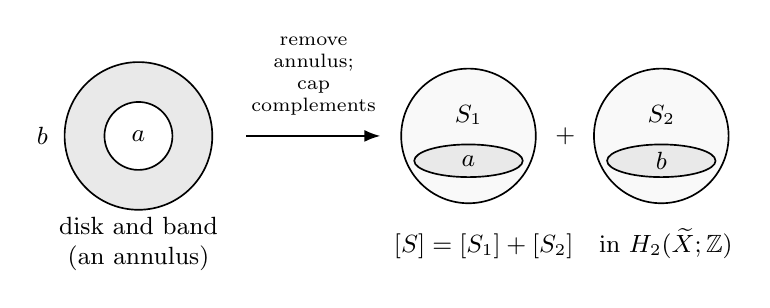
\begin{tikzpicture}[x=0.83cm,y=0.83cm,>=Latex,font=\small,line width=0.6pt]
\begin{scope}
 \fill[gray!17,even odd rule] (0,0) circle (1.13) (0,0) circle (0.52);
 \draw (0,0) circle (1.13);
 \draw (0,0) circle (0.52);
 \node at (0,0) {$a$};
 \node at (-1.47,0) {$b$};
 \node[align=center] at (0,-1.65) {disk and band\\(an annulus)};
\end{scope}
\draw[->] (1.65,0)--(3.7,0);
\node[align=center,font=\scriptsize,anchor=south] at (2.68,0.16) {remove\\annulus;\\cap\\complements};
\begin{scope}[shift={(5.05,0)}]
 \fill[gray!5] (0,0) circle (1.03);
 \draw (0,0) circle (1.03);
 \fill[gray!17] (0,-0.38) ellipse (0.83 and 0.25);
 \draw (0,-0.38) ellipse (0.83 and 0.25);
 \node at (0,-0.38) {$a$};
 \node at (0,0.32) {$S_1$};
\end{scope}
\node at (6.53,0) {$+$};
\begin{scope}[shift={(8,0)}]
 \fill[gray!5] (0,0) circle (1.03);
 \draw (0,0) circle (1.03);
 \fill[gray!17] (0,-0.38) ellipse (0.83 and 0.25);
 \draw (0,-0.38) ellipse (0.83 and 0.25);
 \node at (0,-0.38) {$b$};
 \node at (0,0.32) {$S_2$};
\end{scope}
\node at (6.5,-1.65) {$[S]=[S_1]+[S_2]\quad\text{in }H_2(\widetilde X;\mathbb Z)$};
\end{tikzpicture}


\caption{An inner disk joined to itself by a band forms an annulus. Cutting away the annulus leaves two complementary disks. Capping their new boundaries through the same abstract cone gives two spheres whose homology classes sum to the original class in the universal cover. The labels \(a,b\) indicate the shortened boundary paths; the picture is schematic.}
\label{fig:band-surgery}
\end{figure}

For the essentiality assertion in the third case, illustrated in \Cref{fig:band-surgery}, lift the original sphere map to the universal cover \(\widetilde X\). The map \(K_\Lambda\to X\) has a lift because the cone is simply connected. Choose this lift to agree with the lifted sphere at one point of the annulus. Since the annulus is connected, uniqueness of lifts gives agreement throughout it. Fill both new caps in \(K_\Lambda\) and use this same lift.

With compatible orientations, the original spherical class in \(H_2(\widetilde X;\mathbb Z)\) is the sum of the two capped classes. The difference between the original class and this sum is represented by the annulus together with the reverse caps, all mapping through the contractible cone, so it is zero in homology. Since \(\widetilde X\) is simply connected, the Hurewicz map sending a sphere to its fundamental homology class identifies \(\pi_2(\widetilde X)\) with \(H_2(\widetilde X;\mathbb Z)\)~\cite[Theorem~4.37]{Hatcher2002}. A nonzero original class therefore leaves a nonzero capped class. This uses no prior vanishing of \(\pi_2(X)\).

In every case the retained surface still witnesses the chosen kind of failure, and its total boundary length has strictly decreased. For the split sphere this follows because the total new length over both parts is already smaller; keeping just one part cannot increase it. Collar homotopies restore combinatorial boundaries after the contractions, and further tightening only decreases length. In the exterior cases, the new graph path has the same fixed distinct endpoints. This contradicts the chosen minimum.

Thus every paired occurrence uses a different underlying graph edge from its partner. The minimized picture is now an arrangement of \Cref{def:arrangement}: it has at least one ordinary cyclic boundary, at most one rooted exceptional interval with one break, a full planar inverse-letter pairing, and the reduction condition. \Cref{prop:no-arrangements} excludes it. This proves \Cref{prop:topology}.

\subsection{A finite-dimensional obstruction to torsion}

\begin{corollary}\label{cor:torsion-free}
The universal cover of \(X\) is contractible, and \(G\) is torsion-free.
\end{corollary}
\begin{proof}
The simply connected two-dimensional cover \(\widetilde X\) has \(H_2=0\) by \Cref{prop:topology} and Hurewicz, has \(H_1=0\), and has no cellular homology above dimension two. It is therefore contractible by the homological form of Whitehead's theorem~\cite[Corollary~4.33]{Hatcher2002}.

For completeness, the torsion obstruction can be seen directly from resolutions; compare~\cite[Chapter~VIII, Section~2]{Brown1982}. The augmented cellular chains of \(\widetilde X\) give an exact free \(\mathbb ZG\)-resolution of \(\mathbb Z\) of length two. If \(G\) had a nontrivial finite-order element, a power would generate a cyclic subgroup \(H=\langle g\rangle\) of prime order \(\ell\). Restricting the resolution to \(\mathbb ZH\) preserves freeness, since \(\mathbb ZG\) is free as a left \(\mathbb ZH\)-module on coset representatives.

The cyclic group has the exact periodic resolution
\[
\cdots\longrightarrow\mathbb ZH
 \xrightarrow{\,N\,}\mathbb ZH
 \xrightarrow{\,g-1\,}\mathbb ZH
 \xrightarrow{\,N\,}\mathbb ZH
 \xrightarrow{\,g-1\,}\mathbb ZH
 \longrightarrow\mathbb Z\longrightarrow0,
 \qquad N=1+g+\cdots+g^{\ell-1}.
\]
Exactness follows by comparing the coefficients of \(1,g,\ldots,g^{\ell-1}\): the kernel of \(g-1\) consists of the multiples of \(N\), and the kernel of \(N\) is the augmentation ideal generated by \(g-1\). With trivial coefficients \(\mathbb F_\ell\), all differentials in the corresponding cochain complex vanish. Hence
\(H^k(H;\mathbb F_\ell)\cong\mathbb F_\ell\) in every degree. The comparison theorem for projective resolutions makes this cohomology independent of the chosen resolution~\cite[Chapter~I, Theorem~7.5, p.~24]{Brown1982}. This contradicts the vanishing above degree two forced by the restricted finite-length free resolution.
\end{proof}

\section{The zero divisors}\label{sec:factors}

\begin{proof}[Proof of \Cref{thm:main}]
Use the graphs of \Cref{prop:no-arrangements} and the complex \(X\) constructed in \Cref{sec:topology}. It is finite and two-dimensional. By \Cref{cor:torsion-free}, it is a classifying space for the torsion-free group \(G=\pi_1(X)\), which is finitely presented.

Let \(A'\) be the full vertex set of the component of \(x_A\) and \(B'\) that of the component of \(x_B\). For \(x\in A'\), let \(g_x\in G\) be the label of a path from \(x_A\) to \(x\); for \(y\in B'\), define \(h_y\) using paths from \(x_B\). These labels do not depend on the path, because labels of all closed walks in each component are killed by its cone. We multiply in path order.

Set
\[
\alpha=\sum_{x\in A'}g_x,\qquad
\beta=\sum_{y\in B'}h_y^{-1}
\quad\text{in }\mathbb F_2[G].
\]
Both sums are finite. The root contributes the identity to each. By \Cref{prop:topology}, no other vertex contributes identity, so its coefficient is one in each factor. Thus \(\alpha\ne0\) and \(\beta\ne0\). No assertion about equality between two non-root labels is needed.

On \(A'\times B'\), form the graph of simultaneous steps of a common signed label. A step
\[
x\xrightarrow{t}x',\qquad y\xrightarrow{t}y'
\]
sends \(g_x\) to \(g_xt\) and \(h_y\) to \(h_yt\), and therefore preserves
\[
g_{x'}h_{y'}^{-1}
 =(g_xt)(h_yt)^{-1}
 =g_xh_y^{-1}.
\]
The reverse step has label \(\bar t\). Since full components are used, the degree at \((x,y)\) is the entire number \(|S_x\cap S_y|\), which is odd by \eqref{eq:odd-intersections}. The girth condition excludes loops for the chosen large \(n\); parallel edges would not affect the degree-sum argument.

Every finite connected component of the simultaneous-step graph has an even number of vertices, since the sum of its odd degrees is twice its number of edges. The value \(g_xh_y^{-1}\) is constant on that component, so the component contributes zero to the expansion of \(\alpha\beta\) over \(\mathbb F_2\). Summing over all components gives \(\alpha\beta=0\). This proves \Cref{thm:main} and disproves the universal zero-divisor assertion.
\end{proof}

In particular, \(G\) does not have the unique-product property. The construction
is probabilistic: it proves that suitable finite matchings exist, without
specifying matchings from which a concrete presentation and zero-divisor
factors can be read off.


\bibliographystyle{plain}
\bibliography{references/references}
\end{document}
